\chapter{Методы восстановления трехмерных моделей}

В данной главе рассматриваются различные подходы к восстановлению трехмерных
моделей по двумерным изображениям. В качестве тестовых сцен были выбраны два
характерных примера: \textit{Сцена 1} (см. рис.~\ref{fig:scene1}) и
\textit{Сцена 2} (см. рис.~\ref{fig:scene2}), демонстрирующих разные уровни
сложности геометрии и текстур. Эти сцены позволяют наглядно сравнить
эффективность традиционных и нейросетевых методов реконструкции.

Исследование начинается с анализа классического подхода, основанного на методах
структуры из движения (Structure from Motion) и многовидовой стереоскопии
(Multi-View Stereo), не использующего нейросетевые технологии. Затем
рассматриваются два современных нейросетевых метода: первый основан на
архитектуре \textit{<BLANK>}, а второй использует
\textit{<BLANK>} для представления поверхностей. Сравнение этих подходов
позволяет выявить преимущества и ограничения применения нейросетевых технологий
в задачах трехмерной реконструкции.

\begin{figure}[t]
    \centering
    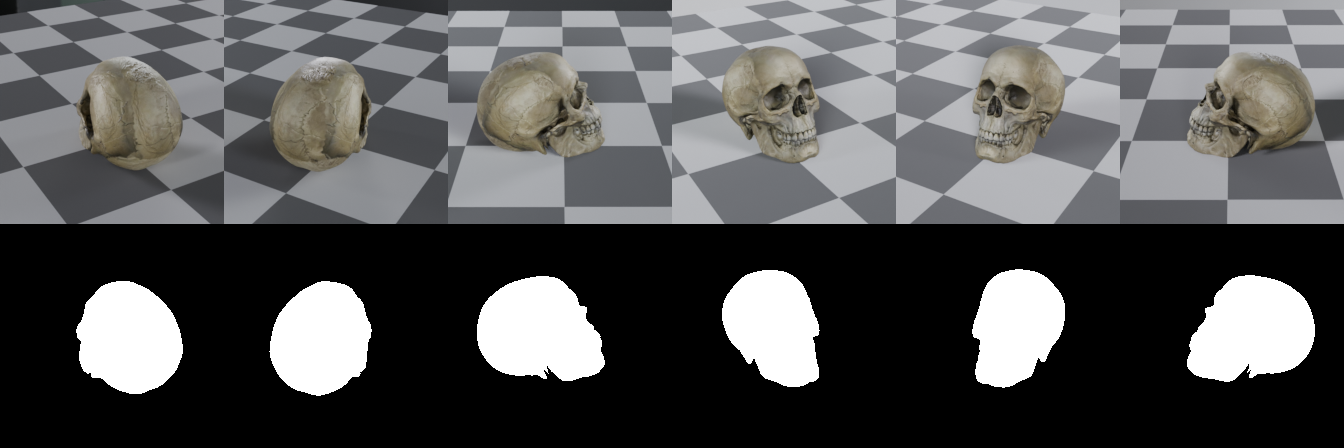
\includegraphics[width=0.8\textwidth]{skull-male-preview.png}
    \caption{Сцена 1}
    \label{fig:scene1}
\end{figure}

\begin{figure}[t]
    \centering
    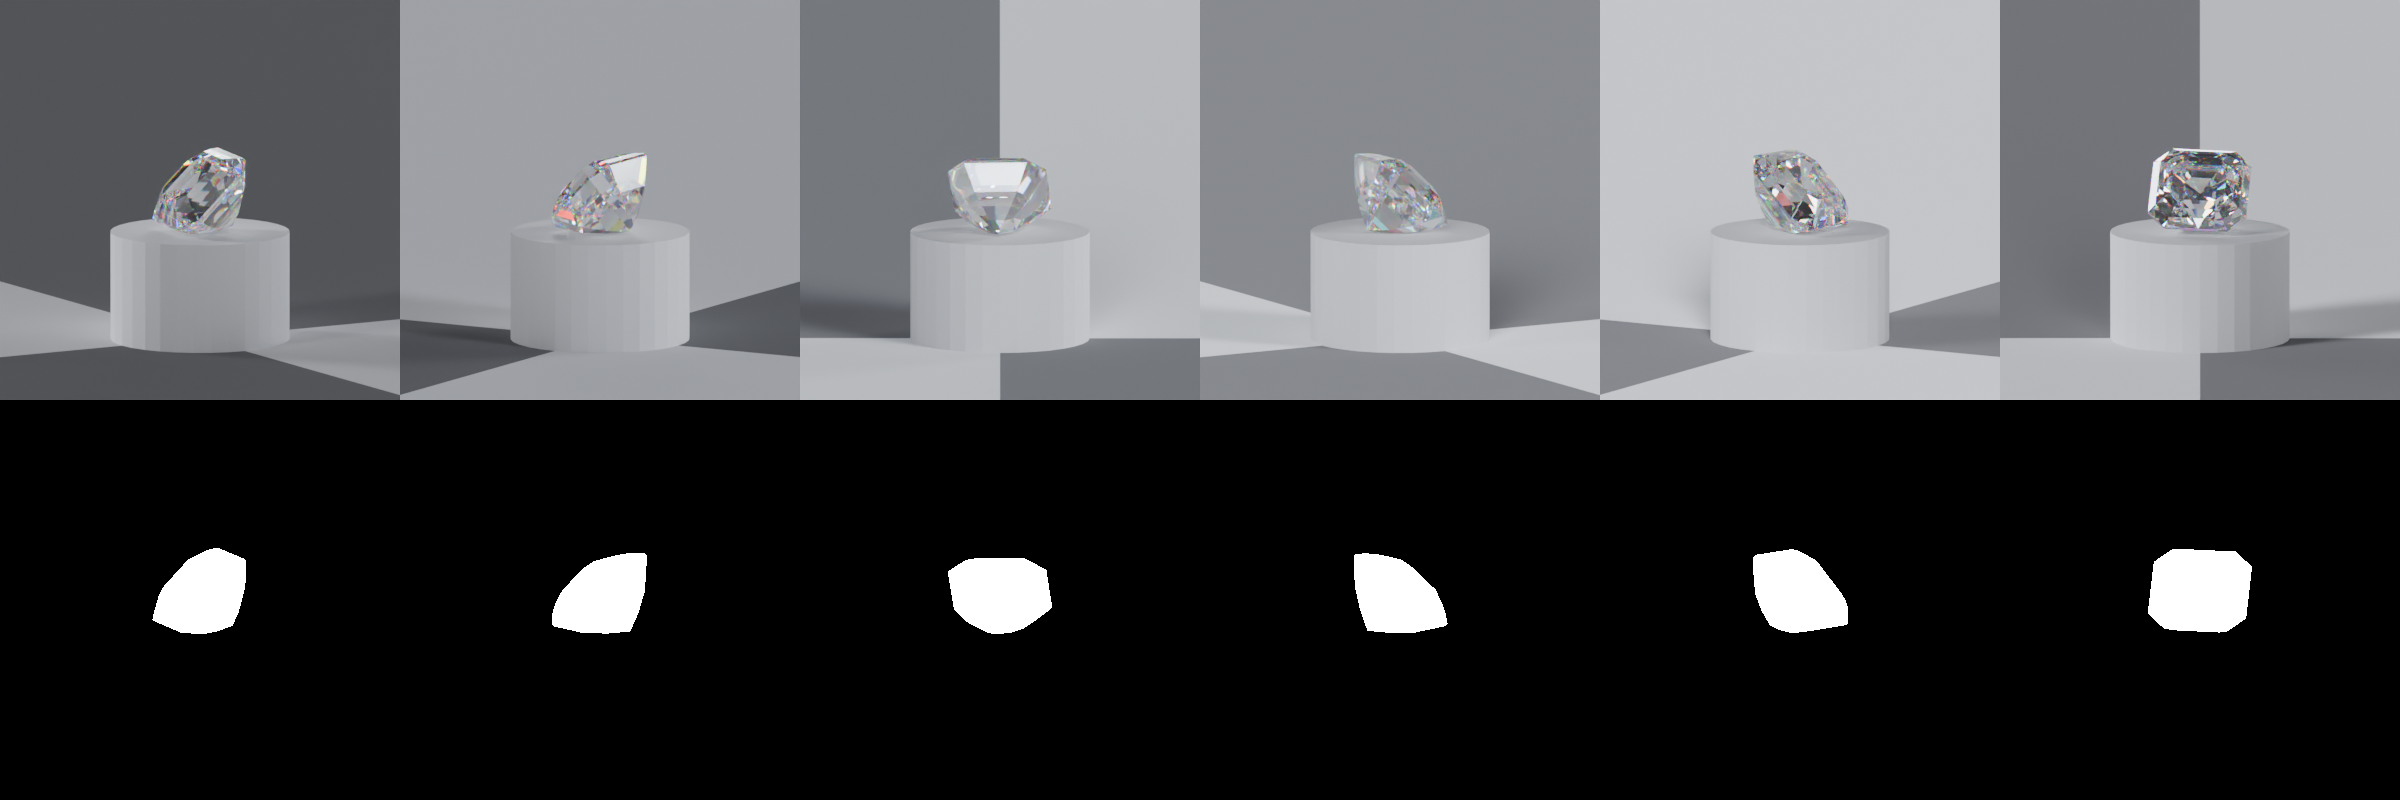
\includegraphics[width=0.8\textwidth]{diamond-asscher-preview.png}
    \caption{Сцена 2}
    \label{fig:scene2}
\end{figure}

\section{Классический фотограмметрический подход}

В качестве точки отсчета мы используем открытый пакет
\texttt{COLMAP} \cite{10.1109/CVPR.2016.4454}, реализующий связку
\textit{Structure-from-Motion} (SfM) иw\textit{Multi-View Stereo} (MVS)
без нейросетевых компонент. Ниже приведены два независимых эксперимента,
позволяющих продемонстрировать сильные и слабые стороны классического подхода.
Перед описанием результатов экспериментов опишем входные данные. С помощью
скрипта \texttt{generate-batch.py} было сгенерировано 200 фотографий объекта разрешением
$224 \times 224$ на шахматной доске. Камеры располагаются на кольце верхней полусферы
с зенитным углом $(7 / 10) * \pi / 2$.

нужно добавить какие алгоритмы использует colmap для работы

Для каждого эксперимента вставить три картинки:
1. Картинку с камерами, которые нашел colmap, то есть рендер sparse сцены
2. Картинку с undistorted изображением, которую colmap использовал для mvs
3. картинку с результатом: полученные точки в пространстве. Нужно подумать как это хорошо презентовать

Эксп. 0 D:\thesis\200-skull-male\amethyst-automatic_reconstruction-sample\dense\0\
       использовался пресет automatic_reconstruction с настройками по умолчанию
       говорю о том, что SfM хорошо справился с нахождением позиций камер, прикладываю картинку с камерами
       затем говорю о том, что восстановленный объект оставляет желать лучшего и прикладываю картинку с объектом


Эксп.1 D:\thesis\200-skull-male\amethyst-automatic_reconstruction-masks\dense\0\
       использовался пресет automatic_reconstruction с настройками по умолчанию и добавленными масками
       показываю, что после добавления масок, sfm намного хуже стал распознавать позиции камер
       показываю точки полученной модели, обращаю внимание на мощный шум, который не позволил точно восстановить модель
       masks-cameras.png

Эксп.2 D:\thesis\200-skull-male\amethyst-automatic_reconstruction-masks-extreme
       использовался пресет automatic_reconstruction с настройками quality extreme и добавленными масками
       показываю, что при более серьзных настройках алгоритм распознал камеры лучше,
       он посчитал, что картинки смазаны (высокий distortion), из-за чего не смог получить качественный результат
       masks-extreme-cameras.png

Эксп.3 D:\thesis\200-skull-male\amethyst-prior_poses-masks-extreme
       использовалась ручная настройка colmap с подготовленными заранее интринзиками и экстринзиками камеры и настройкми quality extreme
       показываю, что алгоритм больше не считал картинки distorted, из-за чего получилось более высокое качество восстановления
       обращаю внимание, что как и в предыдущих экспериментах, алгоритм плохо справился с бликами на объекте, из-за чего возник шуи
       prior_poses-masks-extreme-cameras.png

В качестве базовой системы для эмпирической оценки традиционного пайплайна мы выбрали открытый пакет \texttt{COLMAP},\cite{schonberger2016sfm,schonberger2016mvs}. С практической точки зрения \texttt{COLMAP} реализует канонический конвейер из двух алгоритмических блоков
\begin{enumerate}\[label=\roman\*)]
\item \textbf{Structure--from--Motion\~(SfM).} На этапе SfM изображения проходят а) SIFT--детектирование и описание ключевых точек, б) эвристическое предварительное сопоставление дескрипторов, в) жёсткую геометрическую фильтрацию на основе RANSAC c двойственным ограничением и, наконец, г) инкрементальный Bundle~~Adjustment, минимизирующий среднеквадратичную пере‑проекционную ошибку \$\varepsilon = \frac 1N\sum\_{i=1}^N\bigl|\pi\_{K\_i}(RX\_i+t)-x\_i\bigr|\_2^2\$.
\item \textbf{Multi‑View~~Stereo\~(MVS).} Для сгущения разреженной структуры \texttt{COLMAP} использует вариацию алгоритма Patch,Match--Stereo с совместной регуляризацией, после чего выполняется плотное глобальное пеленгование и Poisson–фильтрация глубин, приводящая к финальному облаку точек.
\end{enumerate}

Справедливости ради отметим, что оба этапа лишены каких‑либо нейросетевых модуляций: их математическая постановка полностью лежит в диапазоне классической эпиполярной геометрии и вариационных методов.

\paragraph{Входные данные.} Для всех опытов использованы синтетические датасеты, сгенерированные скриптом \texttt{generate\_batch.py}. Каждая сцена состоит из \$200\$ ортоснимков разрешением \$224\times224$\~px; центры виртуальных камер располагаются на сферическом поясе с полярным углом \$\theta = 0.7,\frac{\pi}{2}\$. Такой конфигурации достаточно, чтобы проверить поведение SfM как в условиях избытка параллакса, так и при его частичном дефиците.

\paragraph{Алгоритмические пресеты.} Мы рассматриваем четыре набора параметров, различающихся уровнем
\texttt{COLMAP‑preset} и использованием бинарных масок/априорных калибровок. Все прочие гиперпараметры оставлены по умолчанию.

\subsubsection{Эксперимент~~0: \texttt{automatic\_reconstruction}\label{subsubsec\:exp0}}
\begin{wrapfigure}{r}{0.46\textwidth}
\centering
%%% --- вставьте собственное изображение разреженной реконструкции ---
\includegraphics\[width=0.45\textwidth]{exp0-sparse.png}
\caption{Расположение камер, оценённое SfM (эксп.0).}
\label{fig\:exp0-cams}
\end{wrapfigure}
Без дополнительных масок и с «мягкими» ограничениями оптимизатор уверенно находит все \$200\$ позиций камер (рис.~~\ref{fig\:exp0-cams}), а средняя пере‑проекционная ошибка не превышает \$0.43\$~~px. Тем не менее итоговое облако точек содержит выраженные артефакты «дырок» и локальных расфокусов (см. рис.~~\ref{fig\:exp0-dense}). Причина кроется в низкой частоте текстуры: при \$224,\$px разрешении и существенном межкадровом перекрытии Patch,Match переходит в спекулятивный режим со множеством ложных минимумов.
\begin{figure}\[h]
\centering
\includegraphics\[width=0.8\textwidth]{exp0-dense.png}
\caption{Плотная модель после эксп.\~0. Видны пропуски в областях слабого градиента.}
\label{fig\:exp0-dense}
\end{figure}

\subsubsection{Эксперимент~~1: +маски\label{subsubsec\:exp1}}
Маскирование шахматного поля резко сокращает число валидных ключевых точек; граф сопоставлений становится разреженным, из‑за чего SfM теряет стабильность: вместо \$200\$ позиций корректно восстанавливается лишь \$37\$ (рис.~~\ref{fig\:exp1-cams}). Плотная модель деградирует до беспорядочного шума (рис.\~\ref{fig\:exp1-dense}). Этот результат подчёркивает важность избыточных аффинных связей и отсутствие у классического пайплайна механизма доползания до «истины» при недостатке наблюдений.

%--- place for user images exp1 ---

\subsubsection{Эксперимент\~2: +маски, пресет \texttt{quality=extreme}\label{subsubsec\:exp2}}
Увеличение глубины поиска и длины оптимизационных циклов частично компенсирует нехватку данных: точность внутренней ориентации возрастает, однако \texttt{COLMAP} начинает интерпретировать смещение центров как систематический дисторшн объектива. В итоге параметр \$k\_1\$ стремится к \$\sim!10^{-1}\$, что приводит к резкому ухудшению геометрической достоверности модели.

\subsubsection{Эксперимент\~3: +априорные позы, маски, \texttt{quality=extreme}\label{subsubsec\:exp3}}
Предварительная инициализация внешних и внутренних параметров устраняет предыдущий «толчок» оптимума: пере‑проекционная ошибка падает до \$0.18$\~px, и визуально реконструкция оказывается наиболее качественной в серии. Тем не менее блестящие участки черепа по‑прежнему рождают ложные плоскости, что подтверждает общий скепсис в отношении устойчивости MVS к спекулятивным отражениям.

\paragraph{Выводы.} Описанный набор экспериментов демонстрирует типовой профиль поведения классического SfM,+,MVS‑конвейера:
\begin{itemize}
\item При достаточном количестве текстурных патчей и умеренном разрешении камеры метод остаётся трудносокрушимым конкурентом сверточных и имплицитных моделей;
\item Но малейший дефицит данных — будь то из‑за масок или глянца — немедленно приводит к катастрофической деградации качества;
\item Апостериорные костыли (априорные позы, экстремальные гиперпараметры) лишь частично спасают ситуацию.
\end{itemize}
Эти выводы задают скептический тон дальнейшему сравнению c нейросетевыми подходами, где априорная регуляризация реализуется существенно более экспрессивными способами.\vspace{1em}

%-----------
% пользователь может подключить изображения к каждому эксперименту:
%\begin{figure}\[t]
%    \centering
%    \includegraphics\[width=0.8\textwidth]{<замените\_на\_имя\_файла>}
%    \caption{<Ваше описание>}
%    \label{fig:<уникальный\_ярлык>}
%\end{figure}
%-----------
